\tikzstyle{node}=[
    circle,
    draw
]

\begin{tikzpicture}[remember picture]
    \def \n {5}
    \def \radius {2cm}
    \def \margin {11} % margin in angles, depends on the radius

    \foreach \s in {1,...,\n}
    {
    \node[draw, circle] at ({360/\n * (\s - 1)}:\radius) {$P_\s$};
    \draw[<-, >=latex] ({360/\n * (\s - 1)+\margin}:\radius) 
        arc ({360/\n * (\s - 1)+\margin}:{360/\n * (\s)-\margin}:\radius);
    }

    \node[draw, rectangle, minimum width=4cm] at (6,0) {
        \begin{tabular}{c}
            \\
            Process ($P_i$) \\
             \\
            \begin{tikzpicture}[remember picture]
                \node [draw, rectangle, minimum width=3cm, minimum height=1cm] (connector) at (0,0) {\texttt{election\_module}};
            \end{tikzpicture} \\
            \\
            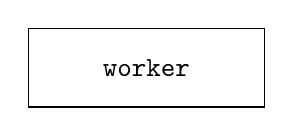
\begin{tikzpicture}[remember picture]
                \node [draw, rectangle, minimum width=3cm, minimum height=1cm] (component) at (0,0) {\texttt{worker}};
            \end{tikzpicture}
            \vspace{0.5em}
        \end{tabular}
        };
    
    \draw[->, >=latex] (3,0.3) -- (connector) node[midway, above, xshift=-0.35cm] {\texttt{left}} ;
    \draw[->, >=latex] (connector) -- (9,0.3) node[midway, above, xshift=0.3cm] {\texttt{right}};
    \draw[<->, >=latex] (component) -- (connector) ;

    \node[] at (0,-2.8) {(a)};
    \node[] at (6,-2.8) {(b)};
\end{tikzpicture}